\documentclass[12 pt]{article}
\usepackage{titling}
\usepackage[a4paper, margin = 1in]{geometry}
\usepackage{graphicx}
\usepackage{caption}
\usepackage{hyperref}
\usepackage{mathtools}
\usepackage{amsmath}
\usepackage{amssymb}
\usepackage{float}
\usepackage{longtable}
\usepackage{fancyhdr}
\usepackage[utf8]{inputenc}
\usepackage[T1]{fontenc}
\setlength{\parindent}{0ex}
\usepackage{setspace}
\usepackage{titlesec}
\usepackage{subcaption}

\setstretch{1.0}

\title{Literature Review – Data processing for the High Granularity Calorimeter at the CMS experiment}
\date{\today}
\author{Stephan Koenigstorfer \\ CID: 01049055 \\ \\ Project code: HEPH-Dauncey-1 \\ Supervisor: Paul Dauncey \\ Assessor: Gavin Davies \\ Word count:} 

\pagestyle{fancy}
\fancyhf{}
\rhead{CID: 01049055}
\lhead{Stephan Koenigstorfer}
\chead{Msci Project}
\cfoot{ \textbf{\thepage}}

\begin{document}
	
	\maketitle

	\begin{figure}[H]
		\centering
		
\includegraphics[width=0.5\textwidth]{imperial_logo.png}
	\end{figure}
	
	\newpage
	\tableofcontents

	\newpage


	\begin{abstract}
		This review is concerned with the Trigger Primitive Generator for the High Granularity Calorimiter at the CMS experiment at the LHC. Specifically, this project is concerned with finding an algorithm to process the low resolution data for every bunch crossing into the energy maps and 3D energy clusters which are required by the Level 1 Trigger as input. This literature review summarises the necessary background material, namely the physics of particle detection and calorimetry, the relevant specifications and limitations of the detector at CMS, the requirements for this Trigger Primitive Generator and reviews particle flow algorithms as candidates for the algorithms in question. 
	\end{abstract}

	\section{Introduction}
		The Large Hardon Collider (LHC) at Cern is undergoing several upgrades over the next decade, with the second long shutdown planned for all of 2019-2020. These upgrades aim to increase the energies which the experiments at the LHC can explore, in order to shed light on new physics. These higher energies will greatly increase the number of events observed, the precision with which these events can be measured and therefore tighten the statistical bounds to measurements of rare events. However, in order to do this, the new detector systems will have to be able to withstand the increased radiation dose without drastic losses in performance. Work is currently being done in order to optimized the plan for these systems. \\ \\
		This project is concerned with the CMS experiment at the LHC, and within this experiment with the Trigger Primitive Generator (TPG) for the High Granularity Calorimeter (HGCAL). Its role is to process preliminary low resolution event data from the Endcap Calorimeter (EC)and pass on to the Level 1 Trigger (L1T) the processed data for the L1T to decide on if this event was interesting. \\
		In order to explore the different options and simulate the processes, background knowledge is needed in the following areas: the physics of particle detection and calorimetry, the specifications and technical limitations of the CMS HGCAL, the requirement on the endcap calorimeter trigger primitive generator (ECT), and existing algorithms which can be used for processing this data. \\ 
		In the following sections, the relevant literature for each of these areas is reviewed and the motivation for this project and the LHC upgrade is explained.
	\section{Motivation for ...}

		\subsection{… Upgrading the LHC}

			The LHC upgrade will allow the exploration of higher energies, and thereby new physics. Specifically, the properties of the Higgs boson will be researched, and the predictions of the standard model (SM) will be tested. This upgrade will increase the luminosity achieved by the LHC and hence how many events are studied. It is expected that the LHC will accumulate about 300 fb$^{-1}$ during its entire existence up to 2023. Through the upgrades it is then expected to accumulate 3000 fb$^{-1}$ by the mid 2030s. This will drastically decrease the time it will take to reduce the statistical errors on measurements of rare events, which would otherwise take more than 10 years to halve\cite{mot}. \\ \\

			By tightening the constraints on theoretical predictions the chance of finding physics beyond the SM is increased. This will allow testing of new theories such as supersymmetry and finding new particles such as weakly interacting massive particles. 

		\subsection{… finding solutions to achieve the requirements for the TPG}
			Finding a way for the TPG to analyze low resolution data of the HGCAL in a way that allows the Trigger to make a correct decision is vital in order to be able read out the interesting events. \\

			The CMS experiment will collect tremendous amounts of data \footnote{The low resolution calorimetry data alone will exceed 5 Tb/s. The high resolution data from all subdetector systems is likely to exceed 100TB/s.} which cannot all be read out and analyzed, since doing so would require too much storage space and computing power. Thus, the L1T system has to make a decision on which events contain interesting physics and then read only these events out to be stored. The system has very limited time to do so, since only small amounts of data can be stored on the detector, and new data is constantly coming in. Thus, the entire L1T system has 12.5$\mu s$ to make this decision, out of which 3.5$\mu s$ are allocated for the ECT data processing. This project is concerned with finding a solution for this requirement. 

		
	\section{The physics of detection and calorimetry}
		\subsection{Particle detection}
			Particle detection occurs over several independent processes \cite{notes13}, as shown in Figure \ref{particle_detecion}. \\
			Charged particles are identified first. This is done by bending their path of motion in a magnetic field, and observing the tracks of ionisation they leave in the detector medium. This also allows for a measurement of their momentum via the radius of the curved track. Since magnetic fields do no work, this detection is non-destructve. \\
		    This is followed by an Electromagnetic Calorimeter, which absorbs electrons and photons by inducing an electron shower (see section \ref{electroshowers}). Both particles leave similar tracks, but can be distinguished by the electron leaving a track in the earlier track detector. All other charged particles will leave only a small deposit. \\
			Next follows a hadronic calorimeter, which absorbs hadrons based on a hadron shower. The only hadrons that are stable enough to survive until they reach the detector are protons, neutrons, K-longs, and sometimes Pions and Kaons. Other hadrons will decay (usually into these more stable hadrons) before reaching the detector material. \\
			Finally, the only semi-stable particle left is the muon, which can then be identified in another magnetic track detector.


			\begin{figure}[H]
				\centering
				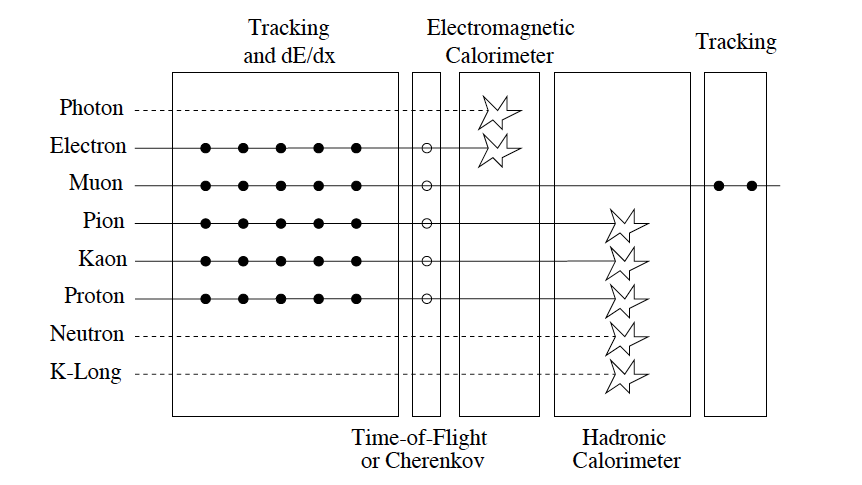
\includegraphics[width=0.9\textwidth]{particle_detection.png}
				\label{particle_detection}
				\caption{Figure showing different detection methods for different particles, as found in \cite{notes13}.}
			\end{figure}

		\subsection{Electromagnetic showers}\label{electroshowers}
			In order to measure the energy of a particle, it is necessary for it to deposit all this energy into the detector material. Fortunately, this process is facilitated by particle showers. An electromagnetic particle shower will create a large number of electrons and photons out of a single high energy photon or electron, making it much easier to measure the energies. \\

			Electromagnetic showers work based on alternating between two phyical processes: electron-positron pair production from $\gamma$s and electrons undergoing bremsstrahlung \cite{notes13}. These usually happen over a characteristic lengthscale $X_0$, called the radiation length, over which one interaction takes place. This shower continues for several lengthscales, until the average electron energy is sufficiently low such that it no longer radiates energy via photons but instead deposits all its energy into the detector material via Boethe-Bloch energy loss.

			A diagram of a shower in such a detector can be seen in Figure \ref{particle_shower}.
			\begin{figure}[H]
				\centering
				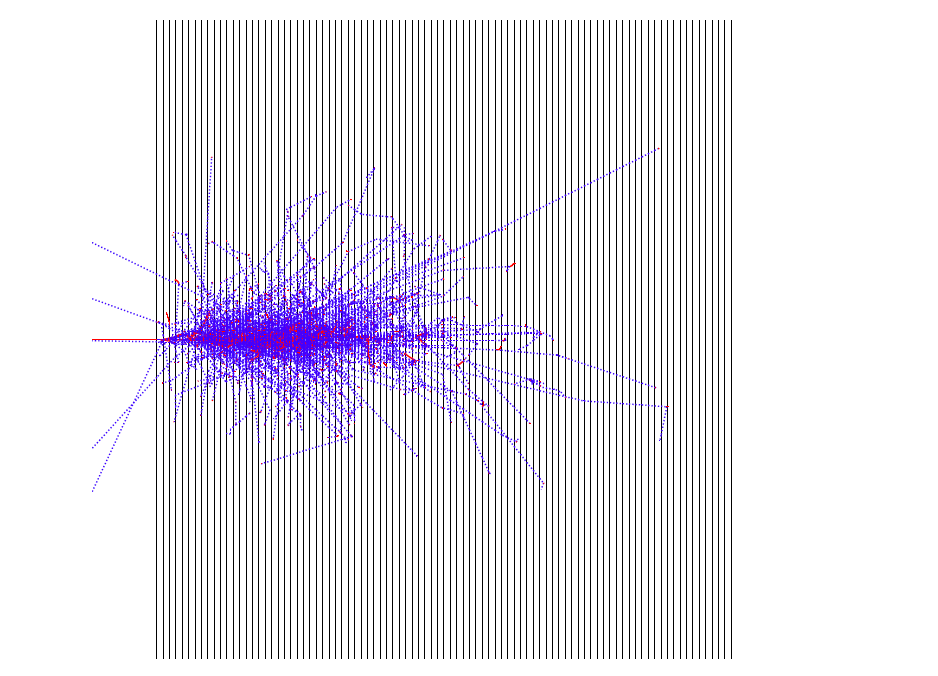
\includegraphics[width=0.9\textwidth]{particle_shower.png}
				\label{particle_shower}
				\caption{Figure showing an electromagnetic particle shower in a detector, as shown in \cite{notes13}.}
			\end{figure}

		\subsection{Hadronic showers}

			Hadronic showers are based on the same principles as electromagnetic showers (see section \ref{electroshowers}), with the difference being that they work via the strong force instead of the elctromagnetic force \cite{}. This increases the hadronic equivalent of the radiation length, since the number density of nuclei is lower than that of electrons. On the other hand, when a hadron does interact with a nucleus, many more hadrons are created. The shower therefore becomes more wide than an electromagnetic shower would. 



		\subsection{Minimum Ionizing Particles (MIPs)}
			A MIP is a useful way of classifying the minimum necessary precision of a detector. As a particle moves through a detector, it positions a certain amount of energy into the detector per unit distance ($\frac{dE}{dx}$), dependent on its momentum, the type of particle and the material it is moving through. At low momenta this ratio decreases with increasing momenta, however, due to relativity it starts to rise again at high momenta. This is called the "relativistic rise", and always causes a minimum in the plot of ($\frac{dE}{dx}$) vs $p$. A particle moving at this momentum is called a MIP, and is the most difficult to detect, since it deposits the least amount of energy into the detector material per distance. \\

			The exact minimum points for different particles are very close together, and hence all particles are treated to bottom out at the same value, such that the MIP can be considered a universal parameter for a given detector material. 

		\subsection{Particle calorimetry}
			In order to measure the energy of a particle, it needs to deposit all its energy into an absorbing material, and this energy increase in then needs to be measured by a detector material \cite{}. In order to do this, the two materials are alternated in layers. A usual choice for the detector material is silicon or a scintillator \footnote{A scintillator design creates photons from ionizing particles and reads out the number of photons via a photomultiplier tube.}, while dense materials such as stainless steel or lead are often chosen for the sborbing material.


		
	\section{Specifications and technical limitations of the CMS HGCAL}
		\subsection{Detector type}	
			The HGCAL consists of 3 different sections \cite{TDR}, the electromagnetic calorimeter and two different hadronic calorimeters. The electromagnetic section uses silicon as the detector material and a lead-stainless steel combination as the absorbing material. The first (inner) hadronic section also uses silicon as a detector material, and stainless steel as the absorbing material, while the second (outer) hadronic section uses stainless steel as the absorbing material and a scintillator design for detection. 
		
		\subsection{Readout system \& electronics}
			The data aquisition system is reads out the measurement from individual hexagonal silicon sensor cells   \cite{TDR} via HGCAL read out chips (HGROCs). The HGROC also sum the individual sensor cells over a larger area called a trigger cell, which is the input for the ECT system. 

			\begin{figure}[H]
				\centering
				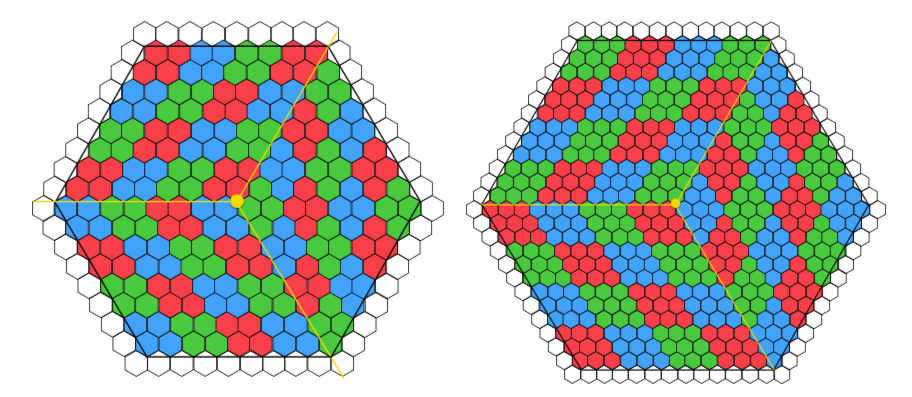
\includegraphics[width=0.9\textwidth]{readout-electronics.png}
				\label{readout}
				\caption{A diagram of the two proposed options for the sensor cells at the CMS HGCAL as found in \cite{TDR}. The total hexagonal wafers are 8'' in diameter, the small hexagons are the individual sensor cells and the colour coded groupings represent the trigger cells. There are currently two sizes being considered for the sensor cells, one being 1.12$cm^2$ (left) and the other 0.52$cm^2$ (right).}
			\end{figure}

			There will be ca. 27,000 such wafers installed in the electromagnetic and hadronic calorimeters of the HGCAL. \\
			The outer layers of the hadronic section will run on a different design \cite{TDR}. They will have the same silicon wafers in the center, but move to a tile based design further outwards from the centre. 



		\subsection{Data transmission}
			The data for the ECT comes from 38 (out of 52) sensitive layers in the endcap calorimeter. The data is then summed over multiple channels, which will constitue one "trigger cell". A selection is made in the frontend electronics (FE) to select only trigger cells above 2 MIP deposits, in order to limit the read out bandwidth to non prohibitive values \cite{itdr}. This selection of trigger cells is the input data for the ECT. In order to get a complete energy measurement, the total energy is also summed over large numbers of trigger cells, which can then be transmitted with far less bandwidth. 

			The ECT then processes the data into 3-D clusters (as stated above), and create an overall energy map in two dimensions. Both of these will form the output of the TPG. The 3D clusters are assumed to have an average size of 200 bits \cite{TDR} and around 200 such clusters exist post selection (threshhold of $E_T$ = 1GeV) per endcap. The are an assumed 1100 energy map bins per endcap, each of which will require 16 bits \cite{TDR}. This yields a total of 60 kbit per endcap per BX, or a resulting bandwidth of 4.8Tb/s. This can be slightly altered since it would just involve an extra optical fibre \cite{TDR}. 
		
		\subsection{Processing power}\label{processing}
			The TPG will receive data directly from the front end electronics of the individual detector layers \cite{TDR} (both the elecromagnetic and the hadronic calorimeters). The processing will happen on Fielf Programmable Gate Arrays (FPGAs) mounted on specifically designed boards, called ATCA boards. Each of these boards can receive up to 96 links, which is the limiting factor in regards to how many boards are needed for a single layer. The electromagnetic layers will need to be read out into 2 boards, while the hadronic layers will need to be read out into single boards. FPGAs are used since they can perform a large number of processes in parallell. The FPGAs run at a clock speed of between 280-440 MHz. 
			\begin{figure}[H]
				\centering
				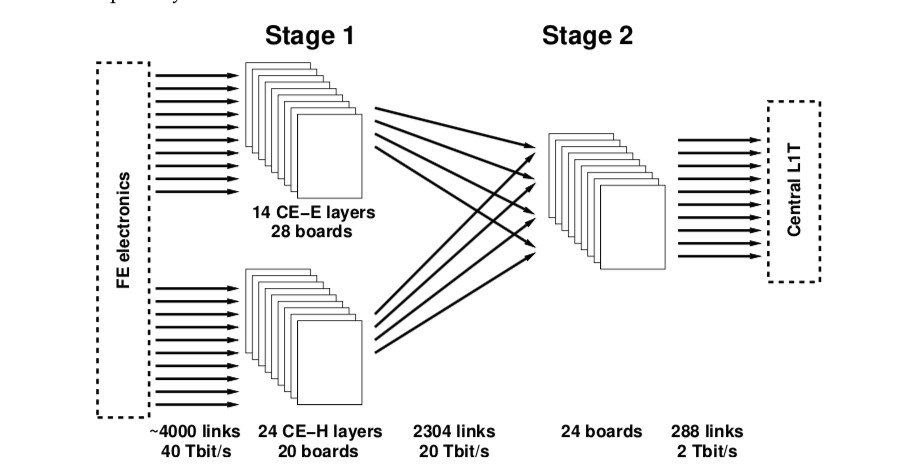
\includegraphics[width=0.9\textwidth]{TPG-stages.png}
				\label{tgp-stages}
				\caption{The two stages of the ECT processing as found in \cite{TDR}. Each board has one large FPGA for processing.}
			\end{figure}

			The processing is structured in 2 stages as can be seen in figure \ref{tgp-stages}. In stage 1 the data is read out from the front end electronics into the first set of 48 boards. Some processing and selection has to take place at this stage, in order to reduce the data to half the amount. The data is then passed on to the second set of 24 time-multiplexed boards, which produce the output of the TPG, which needs to reduce the amount of data by at least an order of magnitude. These boards process 1 out of every 24 bunch crossings (BX), and receive all the data from this BX. The maximum data volume per event will be at 1.2 MBytes, and the average at 0.2MBytes. 

			An identical design will be used for both endcaps of the Calorimeter. 


	\section{Requirements for the ECT}\label{tpg}
		\subsection{Background: How the trigger system works}

			The Level 1 Trigger (L1T) makes the decision on which events are worth analysing and which to discard \cite{TDR} \cite{itdr}. To make this decision, it receives inputs from several TPGs, one for every major detector system\footnote{For an explaination of the subsystems, their roles and acronyms, please see The Phase-2 Upgrade of the CMS Level-1 Trigger: Interim Technical Design Report \cite{itdr}.} \cite{itdr} as shown in figure \ref{l1t_system}. Each one of these TPGs makes an early selection and passes on processed data to the L1T. The L1T then has to make a final decision on weather to accept the event data and save it for further processing, or to discard it \cite{TDR,itdr}. This has to be done within a fixed latency, namely 12.5$\mu s$ \cite{TDR}, which includes roughly 3.5$\mu s$ for the TPGs' decisions. This latency requirement is one of the key challenges to any data processing which is to be done. 

			\begin{figure}[H]
				\centering
				\includegraphics[width=0.9\textwidth]{L1t_system.png}
				\label{l1t_system}
				\caption{The Level 1 Trigger system, as found in \cite{itdr}.}
			\end{figure}

			In the case of this project, the relevant TPG is the Endcap Calorimeter TPG (ECT). The way this is suggested to work is described in the paragraph below, extracted from \cite{itdr}.

			\begin{quotation}
				The ECT data is processed in two stages. The first stage will consider each layer separately, forming two- dimensional (2D) clusters from trigger cells, and summing tower data into a single $\eta$, $\phi$ grid for the particular layer being processed. The second stage will then combine the 2D clusters in depth to form three-dimensional (3D) clusters. It will also combine all the single-layer tower map data with an appropriate weighting into the complete transverse energy tower map. We envisage using time-multiplexing to transfer all the 2D clusters and tower maps for a single bunch crossing into one FPGA. A time multiplexing period of 18 or 24 would be sufficient for this purpose. Preliminary studies of the firmware implementation indicate that trigger primitive generation within 5 $\mu s$ of the bunch crossing is feasible in this architecture, including the time (up to 600 ns) added by the time-multiplexing. The completed tower maps and 3D clusters form the ECT primitives that are transmitted to the L1 trigger.
			\end{quotation}

			The exact method by which this data processing will take place has not yet been decided \cite{itdr,TDR}. 

		\subsection{Output requirements}
			The required output will be 3D energy clusters and energy maps \cite{itdr}. Energy maps will show the distribution of the coarse granularity energy sums from each HG read out chips (HGROC), while the 3D clusters will shope the amount of energy deposited by a particle, and its shape and size from individual trigger cells.

		\subsection{Latency requirements}
			Currently there are 3.5$\mu s$ allocated for processing the ECT data \footnote{The difference in the 3.5 $\mu s$ latency quoted above and the 5 $\mu s$ latency in the paragraph below is the result of the inclusion of the data transmission time of 1.5 $\mu s$}, out of which some time might be necessary to arrange the time multiplexing. This includes the time for both stage 1 \& 2 of the ECT processing (for more information on the ECT structure please see \ref{processing}). 
		

	\section{Algorithms for data processing}
		\subsection{Particle Flow Algorythms (PFAs)}\label{PFAs}
			PFAs provide a useful way to reduce the error on the parts of the calorimeter with less resolution \cite{PFAsInHCAL} \cite{PFAsDualReadout}. This is done by using the detector type with the lowest energy/momentum uncertainty for every particle type, and using the track observed to assign energy deposits in other detector types to the known particle. This is made significantly simpler in the proposed CMS upgrade, due to the high granularity \cite{PFAsInHCAL}.

			Due to the use of PFAs in the L1 trigger system, the ECT output data cannot discard clusters which might be relevant to the tracking of particles. 

	\section{Conclusion}
		The aim of the project is to simulate the environment of the ECT in order to test different algorithms for data processing. By doing this, an algorithm that can produce the required outputs of 3D clusters and energy maps within the required latency of 3.5 $\mu s$ should be found. This might involve the development of some new algorithms, since currently there are rather few algorithms available for such an application. The main questions that remain to be answered are isted below:

		\begin{itemize}
			\item How can the 2D clusters be combined into 3D clusters efficiently?
			\item Is there a more efficient way to process the data than in the currently laid out 2 stage process?
			\item How would the algorithm work that could achive this in the required short timeframe?
		\end{itemize}

	\bibliography{lit_rev}
	\bibliographystyle{ieeetr}{}

\end{document} 

\subsection{L1 Trigger}
			The huge amounts of data produced in each BX cannot all be processed or stored. Therefore, a decision needs to be made for every BX on whether the physics was interesting enough to keep the data or not. The data is then stored in a "buffer", which allows for a processing time of 140BX, or 12.5$\mu s$ \cite{TDR}. 
			The required outcome is a Y/N decision. 
